\chapter{Tools}

This chapter provides a overview of the various tools that are
provided as part of the Ames Stereo Pipeline, and a summary of their
command line options.

\section{stereo}
\label{stereo}

The \texttt{stereo} program is the primary tool of the Ames Stereo
Pipeline. It takes a stereo pair of images that overlap and creates an
output point cloud image that can be processed into a visualizable mesh
or a DEM using \texttt{point2mesh} (section \ref{point2mesh}) and
\texttt{point2dem} (section \ref{point2dem}), respectively.

\medskip

Usage:
\begin{verbatim}
  ISIS 3> stereo [options] <images> [<cameras>] output_file_prefix
\end{verbatim}

Example (for ISIS):
\begin{verbatim}
  stereo file1.cub file2.cub results/run
\end{verbatim}
For ISIS, a .cub file has both image and camera information, as such
no separate camera files are specified.

Example (for Digital Globe Earth images):
\begin{verbatim}
  stereo file1.tif file2.tif file1.xml file2.xml results/run
\end{verbatim}

Multiple input images are also supported (section \ref{multiview}).

This tool is is primarily designed to process USGS ISIS \texttt{.cub}
files and Digital Globe data. However, Stereo Pipeline
does have the capability to process other types of stereo image pairs
(e.g., image files with a CAHVOR camera model from the NASA MER
rovers). If you would like to experiment with these features, please
contact us for more information.

The \texttt{\textit{output\_file\_prefix}} is prepended to all
output data files.  For example, setting \texttt{\textit{output\_file\_prefix}}
to `\texttt{out}' will yield files with names like \texttt{out-L.tif}
and \texttt{out-PC.tif}.  To keep the Stereo Pipeline results organized
in sub-directories, we recommend using an output prefix like
`\texttt{results-10-12-09/out}' for \texttt{\textit{output\_file\_prefix}}.  The
\texttt{stereo} program will create a directory called
\texttt{results-10-12-09/} and place files named \texttt{out-L.tif},
\texttt{out-PC.tif}, etc. in that directory.

\begin{longtable}{|l|p{7.5cm}|}
\caption{Command-line options for stereo}
\label{tbl:stereo}
\endfirsthead
\endhead
\endfoot
\endlastfoot
\hline
Option & Description \\ \hline \hline
\texttt{-\/-help|-h} & Display the help message\\ \hline
\texttt{-\/-threads \textit{integer(=0)}} & Set the number of threads to use. 0 means use as many threads as there are cores.\\ \hline
\texttt{-\/-session-type|-t pinhole|isis|dg|rpc} & Select the stereo session type to use for processing. Usually the program can select this automatically by the file extension.\\ \hline
\texttt{-\/-stereo-file|-s \textit{filename(=./stereo.default)}} & Define the stereo.default file to use.\\ \hline
\texttt{-\/-entry-point|-e integer(=0 to 4)} & Stereo Pipeline entry
point (start at this stage). \\ \hline
\texttt{-\/-stop-point|-e integer(=1 to 5)} & Stereo Pipeline stop point (stop at the stage {\it right before} this value). \\ \hline
\texttt{-\/-corr-seed-mode integer(=0 to 3)} & Correlation seed strategy (section \ref{corr_section}). \\ \hline
\end{longtable}

More information about the stereo.default configuration file can be
found in Appendix \ref{ch:stereodefault} on page
\pageref{ch:stereodefault}.  \texttt{stereo} creates a set
of intermediate files, they are described in Appendix
\ref{chapter:outputfiles} on page \pageref{chapter:outputfiles}.

\subsection{Entry Points}
\label{entrypoints}

The \texttt{stereo -e \textit{number}} option can be used to restart
a {\tt stereo} job partway through the stereo correlation process.
Restarting can be useful when debugging while iterating on {\tt
stereo.default} settings.

Stage 0 (Preprocessing) normalizes the two images and aligns them
by locating interest points and matching them in both images. The
program is designed to reject outlying interest points.  This stage
writes out the pre-aligned images and the image masks.

Stage 1 (Disparity Map Initialization) performs pyramid correlation and builds a rough disparity map that is used to seed the sub-pixel refinement phase.

Stage 2 (Sub-pixel Refinement) performs sub-pixel correlation that
refines the disparity map.

Stage 3 (Outlier Rejection and Hole Filling) performs filtering of the
disparity map and (optionally) fills in holes using an inpainting
algorithm.  This phase also creates a ``good pixel'' map.

Stage 4 (Triangulation) generates a 3D point cloud from the disparity
map.

\subsection{Decomposition of Stereo}
\label{stereo_dec}

The \texttt{stereo}
executable is a python script that makes calls to separate
C++ executables for each entry point.

Stage 0 (Preprocessing) calls \texttt{stereo\_pprc}. Multi-threaded.

Stage 1 (Disparity Map Initialization) calls
\texttt{stereo\_corr}. Multi-threaded.

Stage 2 (Sub-pixel Refinement) class \texttt{stereo\_rfne}. Multi-threaded.

Stage 3 (Outlier Rejection and Hole Filling) calls
\texttt{stereo\_fltr}. Multi-threaded.

Stage 4 (Triangulation) calls \texttt{stereo\_tri}. Multi-threaded,
except for ISIS input data.

All of the sub-programs have the same interface as
\texttt{stereo}. Users processing a large number of stereo pairs on a
cluster may find it advantageous to call these executables in their own
manner. An example would be to run stages 0-3 in order for each stereo
pair. Then run several sessions of \texttt{stereo\_tri} since it is
single-threaded for ISIS.

It is important to note that each of the C++ stereo executables invoked
by \texttt{stereo} have their own command-line options. Those options
can be passed to \texttt{stereo} which will in turn pass them to the
appropriate executable. By invoking each executable with no options, it
will display the list of options it accepts.

As explained in more detail
in section \ref{perform-stereo}, each such option has the same syntax as
used in \texttt{stereo.default}, while being prepended by a double hyphen
(\texttt{-\/-}).  A command line option takes precedence over the same
option specified in \texttt{stereo.default}. Chapter \ref{ch:stereodefault}
documents all options for the individual sub-programs.

\section{stereo\_gui}
\label{stereo_gui}

The \texttt{stereo\_gui} program is a GUI frontend to \texttt{stereo},
and has the same command-line options. It displays
the input images side-by-side. One can zoom in by dragging the
mouse from upper-left to lower-right, and zoom out via the reverse
motion.

By pressing the \texttt{Control} key while dragging the mouse, regions
can be selected in the input images, and then stereo can be run on these
regions from the menu via Run$\rightarrow$Stereo. The \texttt{stereo}
command that is invoked (with parameters for the selected regions) will
be displayed on screen, and can be re-run on a more powerful
machine/cluster without GUI access.

\begin{figure}[h!]
\begin{center}
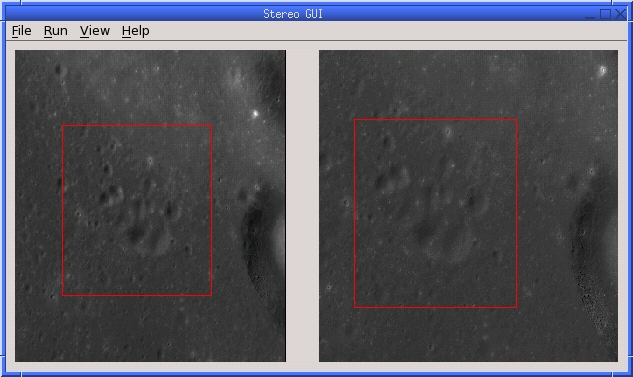
\includegraphics[width=5in]{images/stereo_gui.jpg}
\caption[asp\_gui]{An illustration of stereo\_gui. The \texttt{stereo} command
will be run on the regions selected by red rectangles.}
\label{asp_gui_fig}
\end{center}
\end{figure}

Usage:
\begin{verbatim}
  ISIS 3> stereo_gui [options] <images> [<cameras>] output_file_prefix
\end{verbatim}

This program can be also used as a general-purpose image viewer, being
able to display side-by-side any number of arbitrarily large images with
integer and floating-point pixel values, including ISIS .cub files and
DEMs. In this mode just images need to be passed as inputs, without
cameras or stereo options. \texttt{stereo\_gui} handles large images by
building on disk a pyramid of increasingly coarser subsampled images for
each input image, and displaying the subsampled versions that are
appropriate for the current level of zoom.

Additional navigation options are using the mouse wheel or the +/- to
zoom, and the arrow keys to pan (one should first click to bring into
focus a desired image before using any keys).

This tool can be used to view interest point matches, such as generated
by \texttt{bundle\_adjust} and \texttt{stereo} (only if \texttt{stereo}
was invoked without map-projected images and with homography or affine
epipolar alignemnt). It can also be used to manually create matches
(useful in situations when automatic interest point matching fails due
to large change in illumination) and to delete matches. This functionality
is only enabled if \texttt{stereo\_gui} is invoked like \texttt{stereo},
rather than just with images.


\section{parallel\_stereo}
\label{parallel}

The \texttt{parallel\_stereo} program is a modification of
\texttt{stereo} designed to distribute the stereo processing over
multiple computing nodes. It uses GNU Parallel to manage the jobs, a tool which
is distributed along with Stereo Pipeline. It expects that all nodes
can connect to each other using ssh without password. \texttt{parallel\_stereo}
can also be useful when processing extraterrestrial data on a single computer.
This is because ISIS camera models are restricted to a single thread, but
\texttt{parallel\_stereo} can run multiple processes in parallel to reduce
computation times.

At the simplest, \texttt{parallel\_stereo} can be invoked exactly like stereo,
with the addition of the list of nodes to use (if using multiple nodes).

\begin{verbatim}
  parallel_stereo --nodes-list machines.txt <other stereo options>
\end{verbatim}

If your jobs are launched on a cluster or supercomputer, the name of the
file containing the list of nodes may exist as an environmental
variable. For example, on NASA's Pleiades Supercomputer, which uses the
Portable Batch System (PBS), the list of nodes can be retrieved as
\$PBS\_NODEFILE.

It is important to note that when invoking this tool only stages 1, 2,
and 4 of stereo (section \ref{stereo_dec}) are spread over multiple
machines, with stages 0 and 3 using just one node, as they require
global knowledge of the data. In addition, not all stages of stereo
benefit equally from parallelization. Most likely to gain are stages 1
and 2 (correlation and refinement) which are the most computationally
expensive.

For these reasons, while \texttt{parallel\_stereo} can be called to do
all stages of stereo generation from start to finish in one command, it
may be more resource-efficient to invoke it using a single node for
stages 0 and 3, many nodes for stages 1 and 2, and just a handful of
nodes for stage 4 (triangulation). For example, to invoke the tool
only for stage 2, one uses the options:

\begin{verbatim}
  --entry-point 2 --stop-point 3
\end{verbatim}

\texttt{parallel\_stereo} accepts the following options (any additional
options given to it will be passed to the stereo executables
for each stage).

\begin{longtable}{|l|p{7.5cm}|}
\caption{Command-line options for parallel\_stereo}
\label{tbl:parallelstereo}
\endfirsthead
\endhead
\endfoot
\endlastfoot
\hline
Options & Description \\ \hline \hline
\texttt{-\/-help|-h} & Display the help message.\\ \hline
\texttt{-\/-nodes-list \textit{filename} } & The list of computing nodes,
one per line. If not provided, run on the local machine. \\ \hline
\texttt{-\/-entry-point|-e integer(=0 to 4)} & Stereo Pipeline entry
point (start at this stage). \\ \hline
\texttt{-\/-stop-point|-e integer(=1 to 5)} & Stereo Pipeline stop point
(stop at the stage {\it right before} this value). \\ \hline
\texttt{-\/-corr-seed-mode integer(=0 to 3)} & Correlation seed strategy
(section \ref{corr_section}). \\ \hline
\texttt{-\/-sparse-disp-options \textit{string} } & Options to pass directly
to sparse\_disp (section \ref{sparse-disp}). \\ \hline
\texttt{-\/-verbose } & Display the commands being executed. \\ \hline
\end{longtable}

\subsection{Advanced usage}

The \texttt{parallel\_stereo} tool tries to take advantage of its inside
knowledge of the individual \texttt{stereo} sub-programs to decide
how many threads and processes to use at each stage, and by default, it
it will try to use all nodes to the fullest.

The advanced user can try to gain finer-level control of the tool, as
described below. This may not necessarily result in improved performance
compared to using the default settings.

As an example of using the advanced options, assume that we would like
to launch the refinement and filtering steps only (stages 2 and 3). We
will distribute the refinement over a number of nodes, using 4 processes
on each node, with each process creating 16 threads. For the filtering
stage, which is done in one process on one machine, we want to use 32
threads. The appropriate command is then:

\begin{verbatim}
parallel_stereo --nodes-list machines.txt --processes 4 --threads-multiprocess 16 \
 --threads-singleprocess 32 --entry-point 2 --stop-point 4 <other stereo options>
\end{verbatim}

To better take advantage of these options, the user should know the following.
\texttt{parallel\_stereo} starts a process for every image block, whose
size is by default $2048 \times 2048$ (\texttt{job-size-w} by
\texttt{job-size-h}). On such a block, the correlation, and subpixel
refinement stages will use at most 4 and 64 threads respectively (1 and
16 threads for each $1024 \times 1024$ tile). Triangulation will use at
most 64 threads as well, except for ISIS cameras, when it is
single-threaded due to the limitations of ISIS (we account for the
latter when the number of threads and processes are decided
automatically, but not when these advanced options are used).

\begin{longtable}{|l|p{7.5cm}|}
\caption{Advanced options for parallel\_stereo}
\label{tbl:advancedparallelstereo}
\endfirsthead
\endhead
\endfoot
\endlastfoot
\hline
Options & Description \\ \hline \hline
\texttt{-\/-job-size-w \textit{integer(=2048)}} & Pixel width of input
image tile for a single process. \\ \hline
\texttt{-\/-job-size-h \textit{integer(=2048)}} & Pixel height of input
image tile for a single process. \\ \hline
\texttt{-\/-processes \textit{integer}} & The number of processes to
use per node. \\ \hline
\texttt{-\/-threads-multiprocess \textit{integer}} & The number of threads to use per process.\\ \hline
\texttt{-\/-threads-singleprocess \textit{integer}} & The number of threads to use when running a single process (for pre-processing and filtering).\\ \hline
\end{longtable}

\newpage
\section{bundle\_adjust}
\label{bundleadjust}

The \texttt{bundle\_adjust} program performs bundle adjustment on a
given set of images and cameras. An introduction to bundle adjustment
can be found in chapter \ref{ch:bundle_adjustment}, with an example of
how to use this program in section \ref{baasp}.

This tool can use several algorithms for bundle adjustment. The default is
to use Google's Ceres Solver (\url{http://ceres-solver.org/}).

Usage:
\begin{verbatim}
  bundle_adjust <images> <cameras> <optional ground control points> \
    -o <output prefix> [options]
\end{verbatim}

Example (for ISIS):
\begin{verbatim}
  bundle_adjust file1.cub file2.cub file3.cub -o results/run
\end{verbatim}

Example (for Digital Globe Earth data, using ground control points):
\begin{verbatim}
  bundle_adjust file1.tif file2.tif file1.xml file2.xml gcp_file.gcp \
    --datum WGS_1984 -o results/run
\end{verbatim}

The \texttt{stereo} program can then be told to use the adjusted cameras
via the option \texttt{-\/-bundle-adjust-prefix}.

\begin{longtable}{|l|p{7.5cm}|}
\caption{Command-line options for bundle\_adjust}
\label{tbl:bundleadjust}
\endfirsthead
\endhead
\endfoot
\endlastfoot
\hline
Option & Description \\ \hline \hline
\texttt{-\/-help|-h} & Display the help message. \\ \hline

\texttt{-\/-output-prefix|-o \textit{filename}} & Prefix for output filenames. \\ \hline

\texttt{-\/-bundle-adjuster \textit{string [default: Ceres]}} & Choose a solver from:
Ceres, RobustSparse, RobustRef, Sparse, Ref. \\ \hline

\texttt{-\/-cost-function \textit{string [default: Cauchy]}} & Choose a cost function
from: Cauchy, PseudoHuber, Huber, L1, L2. \\ \hline

\texttt{-\/-robust-threshold \textit{double(=0.5)}} & Set the threshold for robust
cost functions.\\ \hline

\texttt{-\/-datum \textit{string}} & Use this datum (needed only if ground control
points are used). Options: WGS\_1984, D\_MOON (radius is assumed to be 1,737,400 meters), D\_MARS
(radius is assumed to be 3,396,190 meters), etc.  \\ \hline

\texttt{-\/-semi-major-axis \textit{double}} & Explicitly set the datum semi-major axis
in meters (needed only if ground control points are used).\\ \hline
\texttt{-\/-semi-minor-axis \textit{double}} & Explicitly set the datum semi-minor axis
in meters (needed only if ground control points are used).\\ \hline

\texttt{-\/-session-type|-t pinhole|isis|dg|rpc} & Select the stereo
session type to use for processing. Usually the program can select this
automatically by the file extension.\\ \hline

\texttt{-\/-min-matches \textit{integer(=30)}} & Set the minimum number of matches
between images that will be considered. \\ \hline

\texttt{-\/-max-iterations \textit{integer(=100)}} & Set the maximum
number of iterations. \\ \hline

\texttt{-\/-overlap-limit \textit{integer(=3)}} & Limit the number of
subsequent images to search for matches to the current image to this
value.  \\ \hline

\texttt{-\/-camera-weight \textit{double(=1.0)}} &
The weight to give to the constraint that the
camera positions/orientations stay close to
the original values (only for the Ceres solver).
\\ \hline

\texttt{-\/-ip-points-per-tile \textit{int}} &
How many interest points to detect in each $1024^2$ image tile (default: automatic
determination).
\\ \hline

\texttt{-\/-lambda \textit{double}} & Set the initial value of the LM parameter
lambda (ignored for the Ceres solver).\\ \hline

\texttt{-\/-threads \textit{integer(=0)}} & Set the number threads to use. 0 means use the default defined in the program or in the .vwrc file.\\ \hline

\texttt{-\/-report-level|-r \textit{integer=(10)}} & Use a value >= 20 to
get increasingly more verbose output. \\ \hline
\end{longtable}

The \texttt{bundle\_adjust} program will save the obtained adjustments
(rotation and translation) for each camera in plain text files whose
names start with the specified output prefix. This prefix can then be
passed to \texttt{stereo} via the option
\texttt{-\/-bundle-adjust-prefix}.

A number of plain-text files containing ground control points can be
passed as input to \texttt{bundle\_adjust}. Such a file must end with a
.gcp extension, and contain one ground control point per line. Each line
must have the following fields:
\begin{itemize}
\item ground control point id (integer)
\item latitude (in degrees)
\item longitude (in degrees)
\item height above datum (in meters), with the datum itself specified separately
\item $x, y, z$ standard deviations (three positive floating point
  numbers, smaller values suggest more reliable measurements)
\end{itemize}

On the same line, for each image in which the ground control point is
visible there should be:

\begin{itemize}
\item image file name
\item column index in image (float)
\item row index in image (float)
\item column and row standard deviations (two positive floating point
  numbers, smaller values suggest more reliable measurements)
\end{itemize}

The fields can be separated by spaces or commas. Here is a sample representation
of a ground control point measurement:

\begin{verbatim}
5 23.7 160.1 427.1 1.0 1.0 1.0 image1.tif 124.5 19.7 1.0 1.0 image2.tif 254.3 73.9 1.0 1.0
\end{verbatim}

%--------------------------------------------------------------------------
%                           VISUALIZATION TOOLS
%--------------------------------------------------------------------------

\section{point2dem}
\label{point2dem}

The \texttt{point2dem} program produces a GeoTIFF terrain model and/or
an orthographic image from a set of point clouds. The clouds can be
created by the {\tt stereo} command, or be in LAS or CSV format.

Example:\\
\hspace*{2em}\texttt{point2dem \textit{output-prefix}-PC.tif -o stereo/filename -r moon $\backslash$} \\
\hspace*{4em}\texttt{-\/-nodata-value -10000 -n}

This produces a digital elevation model that has been referenced to
the lunar spheroid of 1737.4~km.  Pixels with no data will be set to a
value of -10000, and the resulting \ac{DEM} will be saved in a simple
cylindrical map-projection.  The resulting \ac{DEM} is stored by default as
a one channel, 32-bit floating point GeoTIFF file.

The {\tt -n} option creates an 8-bit, normalized version of the DEM
that can be easily loaded into a standard image viewing application
for debugging.

Another example: \\
\hspace*{2em}\texttt{point2dem \textit{output-prefix}-PC.tif -o stereo/filename -r moon $\backslash$} \\
\hspace*{4em}\texttt{-\/-orthoimage \textit{output-prefix}-L.tif}

This command takes the left input image and orthographically projects
it onto the 3D terrain produced by the Stereo Pipeline.  The resulting
{\tt *-DRG.tif} file will be saved as a GeoTIFF image in a
simple cylindrical map-projection.

Multiple point clouds can be passed as inputs, to be combined into a
single \ac{DEM}. If it is desired to use the \texttt{-\/-orthoimage}
option as above, the clouds need to be specified first, followed by the
\texttt{L.tif} images. Here is an example, which combines together LAS
and CSV point clouds together with an output file from {\tt stereo}:
\begin{verbatim}
  point2dem in1.las in2.csv output-prefix-PC.tif -o combined \
    --dem-spacing 0.001 --nodata-value -32768
\end{verbatim}

\subsection{Comparing with MOLA Data}

When comparing the output of \texttt{point2dem} to laser altimeter
data, like MOLA, it is important to understand the different kinds
of data that are being discussed.  By default, \texttt{point2dem}
returns planetary radius values in meters.  These are often large
numbers that are difficult to deal with.  If you use the \texttt{-r
mars} option, the output terrain model will be in meters of elevation
with reference to the IAU reference spheroid for Mars: 3,396,190~m.
So if a post would have a radius value of 3,396,195~m, in the model
returned with the \texttt{-r mars} option, that pixel would just be 5~m.

You may want to compare the output to MOLA data.  MOLA data is
released in three `flavors,' namely: Topography, Radius, and Areoid.
The MOLA Topography data product that most people use is just the MOLA Radius
product with the MOLA Areoid product subtracted.  Additionally, it is
important to note that all of these data products have a reference
value subtracted from them.  The MOLA reference value is NOT the
IAU reference value, but 3,396,000~m.

In order to compare with the MOLA data, you can do one of two
different things.  You could operate purely in radius space, and
have \texttt{point2dem} create radius values that are directly
comparable to the MOLA Radius data.  You can do this by having
\texttt{point2dem} subtract the MOLA reference value by setting
\texttt{-\/-semi-major-axis 3396000} and \texttt{-\/-semi-minor-axis
3396000}.

To get values that are directly comparable to MOLA Topography data,
you'll need to run \texttt{point2dem} with the option \texttt{-r mars},
then run the ASP tool \texttt{dem\_geoid} (section \ref{demgeoid}). This
program will convert the DEM height values from being relative to the IAU
reference spheroid to being relative to the MOLA Areoid.

\subsection{Post Spacing}
\label{post-spacing}

Recall that \texttt{stereo} creates a point cloud file as its output
and that you need to use \texttt{point2dem} on to create a GeoTIFF that
you can use in other tools.  The point cloud file is the result of
taking the image-to-image matches (which were created from the
kernel sizes you specified, and the subpixel versions of the same,
if used) and projecting them out into space from the cameras, and
arriving at a point in real world coordinates.  Since \texttt{stereo} does
this for every pixel in the input images, the \emph{default} value that
\texttt{point2dem} uses (if you don't specify anything explicitly) is the
input image scale, because there's an `answer' in the point cloud
file for each pixel in the original image.

However, as you may suspect, this is probably not the best value to
use because there really isn't that much `information' in the data.
The true `resolution' of the output model is dependent on a whole
bunch of things (like the kernel sizes you choose to use) but also can
vary from place to place in the image depending on the texture.

The general `rule of thumb' is to produce a terrain model that has a
post spacing of about 3x the input image ground scale.  This is based
on the fact that it is nearly impossible to uniquely identify a single
pixel correspondence between two images, but a 3x3 patch of pixels
provides improved matching reliability.  As you go to numerically
larger post-spacings on output, you're averaging more point data (that
is probably spatially correlated anyway) together.

So you can either use the \texttt{-\/-dem-spacing} argument to
\texttt{point2dem} to do that directly, or you can use your
favorite averaging algorithm to reduce the \texttt{point2dem}-created
model down to the scale you want.

If you attempt to derive science results from an ASP-produced terrain model
with the default \ac{DEM} spacing, expect serious questions from reviewers.

\subsection{Using with LAS or CSV Clouds}

The \texttt{point2dem} program can take as inputs point clouds in LAS
and CSV formats. These differ from point clouds created by stereo by
being, in general, not uniformly distributed.  It is suggested that the
user pick carefully the output resolution for such files
(\texttt{-\/-dem-spacing}). If the output \ac{DEM} turns out to be sparse,
the spacing could be increased, or one could experiment with increasing
the value of \texttt{-\/-search-radius-factor}, which will fill in small
gaps in the output \ac{DEM} by searching further for points in the input
clouds.

It is expected that the input LAS files have spatial reference
information such as WKT data. Otherwise it is assumed that the points
are raw $x,y,z$ values in meters in reference to the planet center.

Unless the output projection is explicitly set when invoking \texttt{point2dem},
the one from the first LAS file will be used.

For LAS or CSV clouds it is not possible to generate intersection error
maps or ortho images.

For CSV point clouds, the option \texttt{-\/-csv-format} must be set. If
such a cloud contains easting, northing, and height above datum, the
option \texttt{-\/-csv-proj4} containing a PROJ.4 string needs to be
specified to interpret this data (if the PROJ.4 string is set, it will be also
used for output DEMs, unless \texttt{-\/-t\_srs} is specified).

\begin{longtable}{|p{8cm}|p{9cm}|}
\caption{Command-line options for point2dem}
\label{tbl:point2dem}
\endfirsthead
\endhead
\endfoot
\endlastfoot
\hline
Options & Description \\ \hline \hline
\texttt{-\/-nodata-value \textit{float(=-3.40282347e+38)}} & Set the nodata value. \\ \hline
\texttt{-\/-use-alpha} & Create images that have an alpha channel. \\ \hline
\texttt{-\/-normalized|-n} & Also write a normalized version of the \ac{DEM} (for debugging). \\ \hline
\texttt{-\/-orthoimage} & Write an orthoimage based on the texture files passed in as inputs (after the point clouds). \\ \hline
\texttt{-\/-errorimage} & Write an additional image whose values represent the triangulation error in meters. \\ \hline
\texttt{-\/-output-prefix|-o \textit{output-prefix}} & Specify the output prefix. \\ \hline
\texttt{-\/-output-filetype|-t \textit{type(=tif)}} & Specify the output file type. \\ \hline
\hline
\texttt{-\/-x-offset \textit{float(=0)}} & Add a horizontal offset to the \ac{DEM}. \\ \hline
\texttt{-\/-y-offset \textit{float(=0)}} & Add a horizontal offset to the \ac{DEM}. \\ \hline
\texttt{-\/-z-offset \textit{float(=0)}} & Add a vertical offset to the \ac{DEM}. \\ \hline
\texttt{-\/-rotation-order \textit{order(=xyz)}} & Set the order of an Euler angle rotation applied to the 3D points prior to \ac{DEM} rasterization. \\ \hline
\texttt{-\/-phi-rotation \textit{float(=0)}} & Set a rotation angle phi. \\ \hline
\texttt{-\/-omega-rotation \textit{float(=0)}} & Set a rotation angle omega. \\ \hline
\texttt{-\/-kappa-rotation \textit{float(=0)}} & Set a rotation angle kappa. \\ \hline
\hline
\texttt{-\/-t\_srs \textit{string}} & Specify the output projection (PROJ.4 string). \\ \hline
\texttt{-\/-reference-spheroid|-r Earth|Moon|Mars} & Set the reference spheroid. This will override manually set datum information. \\ \hline
\texttt{-\/-semi-major-axis \textit{float(=0)}} & Explicitly set the datum semi-major axis in meters.\\ \hline
\texttt{-\/-semi-minor-axis \textit{float(=0)}} & Explicitly set the datum semi-minor axis in meters.\\ \hline
\texttt{-\/-sinusoidal} & Save using a sinusoidal projection. \\ \hline
\texttt{-\/-mercator} & Save using a Mercator projection. \\ \hline
\texttt{-\/-transverse-mercator} & Save using transverse Mercator projection. \\ \hline
\texttt{-\/-orthographic} & Save using an orthographic projection. \\ \hline
\texttt{-\/-stereographic} & Save using a stereographic projection. \\ \hline
\texttt{-\/-oblique-stereographic} & Save using an oblique stereographic projection. \\ \hline
\texttt{-\/-gnomonic} & Save using a gnomonic projection. \\ \hline
\texttt{-\/-lambert-azimuthal} & Save using a Lambert azimuthal projection. \\ \hline
\texttt{-\/-utm \textit{zone}} & Save using a UTM projection with the given zone. \\ \hline
\texttt{-\/-proj-lat \textit{float}} & The center of projection latitude (if applicable). \\ \hline
\texttt{-\/-proj-lon \textit{float}} & The center of projection longitude (if applicable). \\ \hline
\texttt{-\/-proj-scale \textit{float}} & The projection scale (if applicable). \\ \hline
\texttt{-\/-false-northing \textit{float}} & The projection false northing (if applicable). \\ \hline
\texttt{-\/-false-easting \textit{float}} & The projection false easting (if applicable). \\ \hline
\texttt{-\/-dem-spacing|-s \textit{float(=0)}} & Set the output DEM resolution (in target georeferenced units per pixel). If not specified, it will be computed automatically (except for LAS and CSV files). \\ \hline
\texttt{-\/-search-radius-factor \textit{float(=$0$)}} & Multiply this factor by \texttt{dem-spacing} to get the search radius. The DEM height at a given grid point is obtained as a weighted average of heights of all points in the cloud within search radius of the grid point, with the weights given by a Gaussian. Default search radius: max(\texttt{dem-spacing}, default\_dem\_spacing), so the default factor is about 1.\\ \hline

\texttt{-\/-csv-format \textit{string}} & Specify the format of input
CSV files as a list of entries column\_index:column\_type (indices start
from 1). Examples: '1:x 2:y 3:z' (a Cartesian coordinate system with
origin at planet center is assumed, with the units being in meters),
'5:lon 6:lat 7:radius\_m' (longitude and latitude are in degrees, the
radius is measured in meters from planet center), '3:lat 2:lon
1:height\_above\_datum', '1:easting 2:northing 3:height\_above\_datum'
(need to set \texttt{-\/-csv-proj4}; the height above datum is in
meters). Can also use radius\_km for column\_type, when it is again
measured from planet center. \\ \hline

\texttt{-\/-csv-proj4 \textit{string}} & The PROJ.4 string to use to
interpret the entries in input CSV files, if those entries contain
easting, northing, and height above datum. \\ \hline

\texttt{-\/-rounding-error \textit{float(=$1/2^{10}$=$0.0009765625$)}} & How much to round the output DEM and errors, in meters (more rounding means less precision but potentially smaller size on disk). The inverse of a power of 2 is suggested. \\ \hline
\texttt{-\/-dem-hole-fill-len \textit{int(=0)}} &  Maximum dimensions of a hole in the output DEM to fill in, in pixels. \\ \hline
\texttt{-\/-orthoimage-hole-fill-len \textit{int(=0)}} & Maximum dimensions of a hole in the output orthoimage to fill in, in pixels. \\ \hline
\texttt{-\/-remove-outliers-params  \textit{pct (float) factor (float) [default: 75.0 3.0]}} & Outlier removal based on percentage. Points with triangulation error larger than pct-th percentile times factor will be removed as outliers. \\ \hline
\texttt{-\/-max-valid-triangulation-error \textit{float(=0)}} & Outlier removal based on threshold. Points with triangulation error larger than this (in meters) will be removed from the cloud. \\ \hline
\texttt{-\/-median-filter-params \textit{window\_size (int) threshold (double)}} & If the point cloud height at the current point differs by more than the given threshold from the median of heights in the window of given size centered at the point, remove it as an outlier. Use for example 11 and 40.0.\\ \hline
\texttt{-\/-erode-length \textit{length (int)}} & Erode input point clouds by this many pixels at boundary (after outliers are removed, but before filling in holes). \\ \hline
\texttt{-\/-use-surface-sampling \textit{[default: false]}} & Use the older algorithm, interpret the point cloud as a surface made up of triangles and sample it (prone to aliasing).\\ \hline
\texttt{-\/-fsaa  \textit{float(=3)}} & Oversampling amount to perform antialiasing. Obsolete, can be used only in conjunction with \texttt{-\/-use-surface-sampling}. \\ \hline
\texttt{-\/-threads \textit{int(=0)}} & Select the number of processors (threads) to use.\\ \hline
\texttt{-\/-no-bigtiff} & Tell GDAL to not create bigtiffs.\\ \hline
\texttt{-\/-tif-compress None|LZW|Deflate|Packbits} & TIFF compression method.\\ \hline
\texttt{-\/-cache-dir \textit{directory(=/tmp)}} & Folder for temporary files. Normally this need not be changed.\\ \hline
\hline
\texttt{-\/-help|-h} & Display the help message. \\ \hline
\end{longtable}

\section{point2mesh}
\label{point2mesh}

Produces a mesh surface that can be visualized in {\tt osgviewer},
which is a standard 3D viewing application that is part of the open
source OpenSceneGraph package.  \footnote{The full OpenSceneGraph package
is not bundled with the Stereo Pipeline, but the \texttt{osgviewer} program
is.  You can download and install this package separately from
\url{http://www.openscenegraph.org/}.}

Unlike \acp{DEM}, the 3D mesh is not meant to be used as a finished
scientific product.  Rather, it can be used for fast visualization
to create a 3D view of the generated terrain.

The \texttt{point2mesh} program requires a point cloud file and an
optional texture file (\texttt{\textit{output-prefix}-PC.tif} and
normally \texttt{\textit{output-prefix}-L.tif}). When a texture
file is not provided, a 1D texture is applied in the local Z direction
that produces a rough rendition of a contour map.  In either case,
\texttt{point2mesh} will produce a \texttt{\textit{output-prefix}.osgb}
file that contains the 3D model in OpenSceneGraph format.

Two options for \texttt{osgviewer} bear pointing out: the \texttt{-l}
flag indicates that synthetic lighting should be activated for the
model, which can make it easier to see fine detail in the model by
providing some real-time, interactive hillshading.  The \verb#-s#
flag sets the sub-sampling rate, and dictates the degree to which
the 3D model should be simplified.  For 3D reconstructions, this
can be essential for producing a model that can fit in memory.  The
default value is 10, meaning every 10th point is used in the X and
Y directions. In other words that mean only $1/10^2$ of the points
are being used to create the model. Adjust this sampling rate
according to how much detail is desired, but remember that large
models will impact the frame rate of the 3D viewer and affect
performance.

Example:\\
\hspace*{2em}\texttt{point2mesh -s 2 \textit{output-prefix}-PC.tif \textit{output-prefix}-L.tif}

To view the resulting \texttt{\textit{output-prefix}.osgb} file use
\texttt{osgviewer}.

\hspace*{2em}Fullscreen:\\
\hspace*{2em}\texttt{> osgviewer \textit{output-prefix}.osgb}

\hspace*{2em}In a window:\\
\hspace*{2em}\texttt{> osgviewer \textit{output-prefix}.osgb -\/-window 50 50 1000 1000}

Inside \texttt{osgviewer}, the keys L, T, W, and F can be used to toggle on
and off lighting, texture, wireframe, and full-screen modes.  The left, middle, and
right mouse buttons control rotation, panning, and zooming of the
model.

\begin{longtable}{|l|p{10cm}|}
\caption{Command-line options for point2mesh}
\label{tbl:point2mesh}
\endfirsthead
\endhead
\endfoot
\endlastfoot
\hline
Options & Description \\ \hline \hline
\texttt{-\/-help|-h} & Display the help message.\\ \hline
\texttt{-\/-simplify-mesh \textit{float}} & Run OSG Simplifier on mesh, 1.0 = 100\%. \\ \hline
\texttt{-\/-smooth-mesh} & Run OSG Smoother on mesh \\ \hline
\texttt{-\/-use-delaunay} & Uses the delaunay triangulator to create a surface from the point cloud. This is not recommended for point clouds with noise issues. \\ \hline
\texttt{-\/-step|-s \textit{integer(=10)}} & Sampling step size for the mesher. \\ \hline
\texttt{-\/-input-file \textit{pointcloud-file}} & Explicitly specify the input file. \\ \hline
\texttt{-\/-output-prefix|-o \textit{output-prefix}} & Specify the output prefix. \\ \hline
\texttt{-\/-texture-file \textit{texture-file}} & Explicitly specify the texture file. \\ \hline
\texttt{-\/-output-filetype|-t \textit{type(=ive)}} & Specify the output file type. \\ \hline
\texttt{-\/-enable-lighting|-l} & Enables shades and lighting on the mesh. \\ \hline
\texttt{-\/-center} & Center the model around the origin. Use this option if you are experiencing numerical precision issues. \\ \hline
\end{longtable}

\clearpage

\section{dem\_mosaic}
\label{demmosaic}

The program \texttt{dem\_mosaic} takes as input a list of \ac{DEM} files,
optionally erodes pixels at the \ac{DEM} boundaries, and creates a mosaic,
blending the \acp{DEM} where they overlap.

Usage:
\begin{verbatim}
  dem_mosaic [options] <dem files or -l dem_files_list.txt> -o output_file_prefix
\end{verbatim}

The input \ac{DEM} can either be set on the command line, or if there are too
many they can be listed in a text file (one per line) and that file can
be passed to the tool.

The output mosaic is written as non-overlapping tiles with desired tile
size, with the size set either in pixels or in georeferenced (projected)
units. The default tile size is large enough that normally the entire
mosaic is saved as one tile.

Individual tiles can be saved via the \texttt{-\/-tile-index} option
(the tool displays the total number of tiles when it is being run). As
such, separate processes can be invoked for individual tiles for
increased robustness and perhaps speed.

The output mosaic tiles will be named <output prefix>-tile-<tile
index>.tif, where <output prefix> is an arbitrary string. For example,
if it is set to \texttt{results/output}, all the tiles will be in the
\texttt{results} directory. The tile names will be adjusted accordingly
if one of the \texttt{-\/-first}, \texttt{-\/-last}, \texttt{-\/-min},
etc. options is invoked (see below).

By the default, the output mosaicked \ac{DEM} will use the same grid size and
projection as the first input \ac{DEM}. These can be changed via the
\texttt{-\/-tr} and \texttt{-\/-t\_srs} options.

Instead of blending, \texttt{dem\_mosaic} can compute the image of
first, last, minimum, maximum, mean, median, and count of all
encountered valid \ac{DEM} heights at output grid points. For the
``first'' and ``last'' operations, we use the order in which \acp{DEM}
were passed in.

\begin{longtable}{|l|p{10cm}|}
\caption{Command-line options for dem\_mosaic}
\label{tbl:demmosaic}
\endfirsthead
\endhead
\endfoot
\endlastfoot
\hline
Options & Description \\
\hline \hline

\texttt{-l | -\/-dem-list-file \textit{string}}  &
Text file listing the DEM files to mosaic, one per line.
\\ \hline
\texttt{-o | -\/-output-prefix  \textit{string} } &
Specify the output prefix.
\\ \hline
\texttt{-\/-tile-size \textit{integer(=1000000)}} &
The maximum size of output DEM tile files to write, in pixels.
\\ \hline
\texttt{-\/-tile-index \textit{integer}} &
The index of the tile to save (starting from zero). When this program is invoked, it will print  out how many tiles are there. Default: save all tiles.
\\ \hline
\texttt{-\/-erode-length \textit{integer(=0)} }  &
Erode input DEMs by this many pixels at boundary before mosaicking them.
\\ \hline
\texttt{-\/-blending-length \textit{integer(=200)}} &
Larger values of this number (measured in input DEM pixels) may result
in smoother blending while using more memory and computing time.
\\ \hline
\texttt{-\/-tr \textit{double}  } &
Output DEM resolution in target georeferenced units per pixel. Default: use the same resolution as the first DEM to be mosaicked.
\\ \hline
\texttt{-\/-t\_srs \textit{string} } &
Specify the output projection (PROJ.4 string). Default: use the one from the first DEM to be mosaicked.
\\ \hline
\texttt{-\/-t\_projwin \textit{xmin ymin xmax ymax} } &
Limit the mosaic to this region, with the corners given in georeferenced coordinates (xmin ymin xmax ymax). Max is exclusive.
\\ \hline
\texttt{-\/-weights-blur-sigma \textit{integer (=5)} } &
The standard deviation of the Gaussian used to blur the weights. Higher value results in smoother weights and blending.
\\ \hline
\texttt{-\/-weights-exponent \textit{integer (=1)} } &
The weights used to blend the DEMs should increase away from the boundary as a power with this exponent.
\\ \hline
\texttt{-\/-georef-tile-size \textit{double}} &
Set the tile size in georeferenced (projected) units (e.g., degrees or meters).
\\ \hline
\texttt{-\/-output-nodata-value \textit{double}} &
No-data value to use on output. Default: use the one from the first DEM to be mosaicked.
\\ \hline

\texttt{-\/-first}
& Keep the first encountered DEM value (in the input order).
\\ \hline

\texttt{-\/-last}
& Keep the last encountered DEM value (in the input order).
\\ \hline

\texttt{-\/-min}
& Keep the smallest encountered DEM value.
\\ \hline

\texttt{-\/-max}
& Keep the largest encountered DEM value.
\\ \hline

\texttt{-\/-mean}
& Find the mean DEM value.
\\ \hline

\texttt{-\/-stddev}
& Find the standard deviation of DEM values.
\\ \hline

\texttt{-\/-median}
& Find the median DEM value (this can be memory-intensive, fewer threads are suggested).
\\ \hline

\texttt{-\/-count}
& Each pixel is set to the number of valid DEM heights at that pixel.
\\ \hline

\texttt{-\/-threads \textit{integer(=4)}}
& Set the number of threads to use.
\\ \hline
\texttt{-\/-help|-h} & Display the help message.
\\ \hline
\end{longtable}

\clearpage

\section{dem\_geoid}
\label{demgeoid}

This tool takes as input a \ac{DEM} whose height values are relative to the
datum ellipsoid, and adjusts those values to be relative to the
equipotential surface of the planet (geoid on Earth, and areoid on
Mars). The program can also apply the reverse of this adjustment. The
adjustment simply subtracts from the DEM height the geoid height
(correcting, if need be, for differences in dimensions between the DEM
and geoid datum ellipsoids).

Three geoids and one areoid are supported. The Earth geoids are: EGM96
and EGM2008, relative to the WGS84 datum ellipsoid
(\url{http://earth-info.nga.mil/GandG/wgs84/gravitymod/egm96/egm96.html},
\url{http://earth-info.nga.mil/GandG/wgs84/gravitymod/egm2008/egm08_wgs84.html})
and NAVD88, relative to the NAD83 datum ellipsoid
(\url{http://www.ngs.noaa.gov/GEOID/GEOID09/}).

The Mars areoid is MOLA MEGDR
(\url{http://geo.pds.nasa.gov/missions/mgs/megdr.html}). When importing
it into ASP, we adjusted the areoid height values to be relative to
the IAU reference spheroid for Mars of radius 3,396,190~m, to be
consistent with the DEM data produced by ASP. The areoid at that source was
relative to the Mars radius of 3,396,000~m.

\begin{longtable}{|l|p{10cm}|}
\caption{Command-line options for dem\_geoid}
\label{tbl:demgeoid}
\endfirsthead
\endhead
\endfoot
\endlastfoot
\hline
Options & Description \\ \hline \hline
\texttt{-\/-help|-h} & Display the help message.\\ \hline
\texttt{-\/-nodata-value \textit{float(=-32768)}} & The value of no-data pixels, unless specified in the DEM. \\ \hline
\texttt{-\/-geoid \textit{string}} & Specify the geoid to use for Earth WGS84 DEMs.
                               Options: EGM96, EGM2008. Default: EGM96. \\ \hline
\texttt{-\/-output-prefix|-o \textit{filename}} & Specify the output file prefix. \\ \hline
\texttt{-\/-double} & Output using double precision (64 bit) instead of float (32 bit).\\ \hline
\texttt{-\/-reverse-adjustment} & Go from DEM relative to the geoid/areoid to DEM relative to the datum ellipsoid.\\ \hline
\end{longtable}

\section{dg\_mosaic}
\label{dgmosaic}

This tool can be used when processing Digital Globe Imagery (chapter
\ref{ch:dg_tutorial}). A Digital Globe satellite may take a
picture, and then split it into several images and corresponding camera
XML files. \texttt{dg\_mosaic} will mosaic these images into a single
file, and create the appropriate combined camera XML file.

Digital Globe camera files contain, in addition to the original camera
models, their RPC approximations (section
\ref{rpc}). \texttt{dg\_mosaic} outputs both types of combined
models. The combined RPC model can be used to map-project the mosaicked
images with the goal of computing stereo from them (section
\ref{mapproj-example}).

The tool needs to be applied twice, for both the left and right image sets.

\texttt{dg\_mosaic} can also reduce the image resolution while creating the
mosaics (with the camera files modified accordingly).


\begin{longtable}{|l|p{10cm}|}
\caption{Command-line options for dg\_mosaic}
\label{tbl:dgmosaic}
\endfirsthead
\endhead
\endfoot
\endlastfoot
\hline
Options & Description \\ \hline \hline
\texttt{-\/-help|-h} & Display the help message.\\ \hline
\texttt{-\/-reduce-percent \textit{integer(=100)}} &
Render a reduced resolution image and XML based on this percentage. \\ \hline
\texttt{-\/-skip-rpc-gen \textit{[default: false]}} &
Skip RPC model generation.\\ \hline
\texttt{-\/-rpc-penalty-weight \textit{float(=0.1)}} &
The weight to use to penalize higher order RPC coefficients when generating the combined RPC model. Higher penalty weight results in smaller such coefficients.\\ \hline
\texttt{-\/-output-prefix \textit{string}} & The prefix for the output .tif and .xml files. \\ \hline
\texttt{-\/-band \textit{integer}} & Which band to use (for multi-spectral images). \\ \hline
\texttt{-\/-input-nodata-value \textit{float}} & Nodata value to use on input; input pixel values less than or equal to this are considered invalid. \\ \hline
\texttt{-\/-output-nodata-value \textit{float}} & Nodata value to use on output. \\ \hline

\texttt{-\/-preview } & Render a small 8 bit png of the input for preview. \\ \hline
\texttt{-\/- \textit{dry-run|-n}} & Make calculations, but just print out the commands. \\ \hline
\end{longtable}

\clearpage

\section{mapproject}
\label{mapproject}

The tool \texttt{mapproject} is used to map-project a camera image onto
a DEM. The obtained images can be used, for example, to visualize how
camera images would look when projected onto the ground obtained by
doing stereo of these images (ideally, if there were no correlation or
triangulation error, the images would project perfectly). The tool can
also be used to compute stereo from the obtained map-projected images;
this functionality is currently supported only with RPC models (section
\ref{mapproj-example}).

\texttt{mapproject} supersedes the older
\texttt{orthoproject} tool, which could map-project only with ISIS and
pinhole camera models (the latter program is still being kept for a few
releases for backward compatibility). We ported all features of
\texttt{orthoproject} except for projecting of vector imagery (for
example, RGB pixel data).

Any program using ISIS cameras must be single-threaded, due to the
limitations of ISIS. To overcome this, \texttt{mapproject} when invoked
for ISIS images sprawns multiple processes, each working on individual
tiles, then mosaics the results.

Examples:
\begin{verbatim}
mapproject -t isis DEM.tif image.cub  output-IMG.tif --ppd 256
\end{verbatim}

\begin{verbatim}
mapproject -t rpc DEM.tif image.tif image.xml output-IMG.tif --tr 20
\end{verbatim}

\begin{longtable}{|l|p{10cm}|}
\caption{Command-line options for mapproject}
\label{tbl:mapproject}
\endfirsthead
\endhead
\endfoot
\endlastfoot
\hline
Options & Description \\ \hline \hline
\texttt{-\/-nodata-value \textit{float(=-32768)}} & No-data value to use unless specified in the input image. \\ \hline
\texttt{-\/-t\_srs} & Specify the output projection (PROJ.4 string). If not provided, use the one from the DEM. \\ \hline
\texttt{-\/-tr \textit{float}} & Set the output file resolution in target
  georeferenced units per pixel. \\ \hline
\texttt{-\/-mpp \textit{float}} & Set the output file resolution in meters per
pixel. \\ \hline
\texttt{-\/-ppd \textit{float}} & Set the output file resolution in pixels per
degree. \\ \hline
\texttt{-\/-session-type|-t pinhole|isis|rpc} & Select the stereo
session type to use for processing. Choose 'rpc' if it is desired to later do stereo with the 'dg' session. \\ \hline
\texttt{-\/-t\_projwin \textit{xmin ymin xmax ymax}} & Limit the map-projected image to this region, with the corners given in georeferenced coordinates (xmin ymin xmax ymax). Max is exclusive. \\ \hline
\texttt{-\/-t\_pixelwin \textit{xmin ymin xmax ymax}} & Limit the map-projected image to this region, with the corners given in pixels (xmin ymin xmax ymax). Max is exclusive. \\ \hline
\texttt{-\/-bundle-adjust-prefix \textit{string}} & Use the camera
adjustment obtained by previously running bundle\_adjust with this
output prefix. \\ \hline
\texttt{-\/-threads \textit{int(=0)}} & Select the number of processors (threads) to use.\\ \hline
\texttt{-\/-no-bigtiff} & Tell GDAL to not create bigtiffs.\\ \hline
\texttt{-\/-tif-compress None|LZW|Deflate|Packbits} & TIFF compression method.\\ \hline
\texttt{-\/-cache-dir \textit{directory(=/tmp)}} & Folder for temporary files. Normally this need not be changed.\\ \hline
\texttt{-\/-help|-h} & Display the help message. \\ \hline
\end{longtable}

\clearpage

\section{disparitydebug}
\label{disparitydebug}

The \texttt{disparitydebug} program produces output images for
debugging disparity images created from \verb#stereo#. The {\tt
stereo} tool produces several different versions of the disparity
map; the most important ending with extensions \verb#*-D.tif# and
\verb#*-F.tif#. (see Appendix \ref{chapter:outputfiles} for more
information.)  These raw disparity map files can be useful for
debugging because they contain raw disparity values as measured by
the correlator; however they cannot be directly visualized or opened
in a conventional image browser.  The \verb#disparitydebug# tool
converts a single disparity map file into two normalized TIFF image
files (\verb#*-H.tif# and \verb#*-V.tif#, containing the horizontal
and vertical, or line and sample, components of disparity, respectively)
that can be viewed using any image display program.

The {\tt disparitydebug} program will also print out the range of
disparity values in a disparity map, that can serve as useful summary
statistics when tuning the search range settings in the
{\tt stereo.default} file.

\begin{longtable}{|l|p{10cm}|}
\caption{Command-line options for disparitydebug}
\label{tbl:disparitydebug}
\endfirsthead
\endhead
\endfoot
\endlastfoot
\hline
Options & Description \\ \hline \hline
\texttt{-\/-help|-h} & Display the help message\\ \hline
\texttt{-\/-input-file \textit{filename}} & Explicitly specify the input file \\ \hline
\texttt{-\/-output-prefix|-o \textit{filename}} & Specify the output file prefix \\ \hline
\texttt{-\/-output-filetype|-t \textit{type(=tif)}} & Specify the output file type \\ \hline
\texttt{-\/-float-pixels} & Save the resulting debug images as 32 bit floating point files (if supported by the selected file type) \\ \hline
\end{longtable}

\section{orbitviz}
\label{orbitviz}

Produces a Google Earth \ac{KML} file useful for visualizing camera
position. The input for this tool is one or more \texttt{*.cub} files.

\begin{figure}[!b]
  \begin{center}
  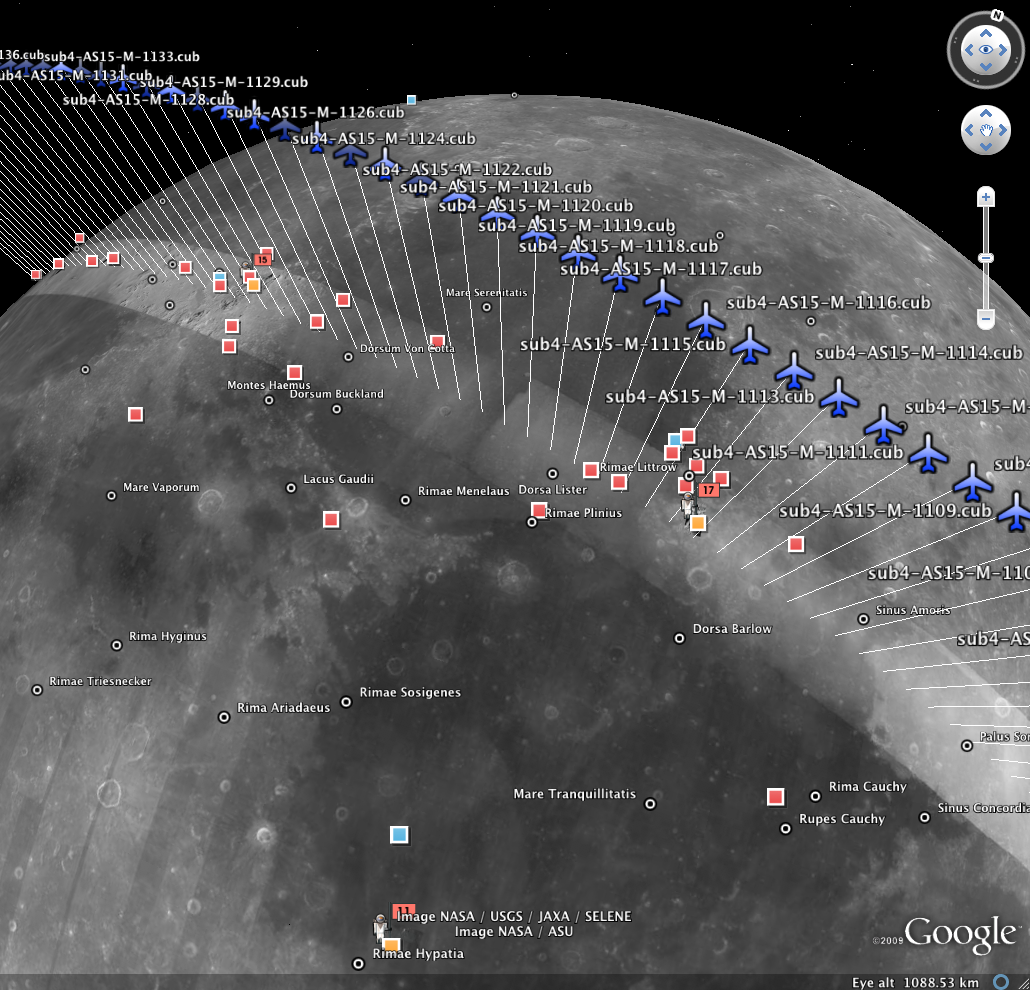
\includegraphics[width=6in]{images/orbitviz_ge_result.png}
  \end{center}
  \caption{ Example of a \ac{KML} visualization produced with {\tt
      orbitviz} depicting camera locations for the Apollo 15 Metric
    Camera during orbit 33 of the Apollo command module.}
  \label{fig:orbitviz_example}
\end{figure}

\begin{longtable}{|l|p{10cm}|}
\caption{Command-line options for orbitviz}
\label{tbl:orbitviz}
\endfirsthead
\endhead
\endfoot
\endlastfoot
\hline
Options & Description \\ \hline \hline
\texttt{-\/-help|-h} & Display the help message\\ \hline
\texttt{-\/-output|-o \textit{filename(=orbit.kml)}} & Specifies the output file name \\ \hline
\texttt{-\/-scale|-s \textit{float(=1)}} & Scale the size of the coordinate axes by this amount. Ex: To scale axis sizes up to Earth size, use 3.66 \\ \hline
\texttt{-\/-use\_path\_to\_dae\_model|-u \textit{fullpath}} & Use this dae model to represent camera location. \emph{Google Sketch up can create these.} \\ \hline
\end{longtable}

\clearpage

\section{cam2map4stereo.py}
\label{cam2map4stereo}

This program takes similar arguments as the ISIS3 \texttt{cam2map} program,
but takes two input images.  With no arguments, the program determines
the minimum overlap of the two images, and the worst common resolution,
and then map-projects the two images to this identical area and resolution.

The detailed reasons for doing this, and a manual step-by-step walkthrough of
what \texttt{cam2map4stereo.py} does is provided in the discussion on aligning images on page \pageref{sec:AligningImages}.

The \texttt{cam2map4stereo.py} is also useful for selecting a subsection and/or reduced resolution portion of the full image.  You can inspect a raw camera geometry image in qview after you have run \texttt{spiceinit} on it, select the latitude and longitude ranges, and then use \texttt{cam2map4stereo.py}'s \texttt{-\/-lat}, \texttt{-\/-lon}, and optionally \texttt{-\/-resolution} options to pick out just the part you want.

Use the \texttt{-\/-dry-run} option the first few times to get an idea of what \texttt{cam2map4stereo.py} does for you.

\begin{longtable}{|l|p{10cm}|}
\caption{Command-line options for cam2map4stereo.py}
\label{tbl:bundlevis}
\endfirsthead
\endhead
\endfoot
\endlastfoot
\hline
Options & Description \\ \hline \hline
\texttt{-\/-help|-h} & Display the help message. \\ \hline
\texttt{-\/-manual} & Read the manual. \\ \hline
\texttt{-\/-map=\textit{MAP}|-m \textit{MAP}} & The mapfile to use for \texttt{cam2map}. \\ \hline
\texttt{-\/-pixres=\textit{PIXRES}|-p \textit{PIXRES}} & The pixel resolution mode to use for \texttt{cam2map}. \\ \hline
\texttt{-\/-resolution=\textit{RESOLUTION}|-r \textit{RESOLUTION}} & Resolution of the final map for \texttt{cam2map}. \\ \hline
\texttt{-\/-interp=\textit{INTERP}|-i \textit{INTERP}} & Pixel interpolation scheme for \texttt{cam2map}. \\ \hline
\texttt{-\/-lat=\textit{LAT}|-a \textit{LAT}} & Latitude range for \texttt{cam2map}, where \texttt{LAT} is of the form \textit{min:max}.  So to specify a latitude range between -5 and 10 degrees, it would look like \texttt{-\/-lat=-5:10}. \\ \hline
\texttt{-\/-lon=\textit{LON}|-o \textit{LON}} & Longitude range for \texttt{cam2map}, where \texttt{LON} is of the form \textit{min:max}.  So to specify a longitude range between 45 and 47 degrees, it would look like \texttt{-\/-lon=40:47}. \\ \hline
\texttt{-\/-dry-run|-n} & Make calculations, and print the \texttt{cam2map} command that would be executed, but don't actually run it.\\ \hline
\texttt{-\/-suffix|-s} & Suffix that gets inserted in the output file names, defaults to `map'.\\ \hline
\end{longtable}

\clearpage

\section{point2las}
\label{point2las}

This tool can be used to convert point clouds generated by ASP to the
public LAS format for interchange of 3-dimensional point cloud data.

\begin{longtable}{|l|p{10cm}|}
\caption{Command-line options for point2las}
\label{tbl:point2las}
\endfirsthead
\endhead
\endfoot
\endlastfoot
\hline
Options & Description \\ \hline \hline
\texttt{-\/-help|-h} & Display the help message.\\ \hline
\texttt{-\/-reference-spheroid|-r Earth|Moon|Mars} & "Set the reference spheroid [Earth, Moon, Mars]. This will create a geo-referenced LAS file in respect to the spheroid. For Earth, the WGS84 datum is used. \\ \hline
\texttt{-\/-t\_srs \textit{string}} & Specify the output projection (PROJ.4 string). \\ \hline
\texttt{-\/-compressed} &
Compress using laszip. \\ \hline
\texttt{-\/-output-prefix|-o \textit{filename}} & Specify the output file prefix. \\ \hline
\texttt{-\/-threads \textit{integer(=0)}} & Set the number threads to use. 0 means use the default defined in the program or in the .vwrc file.\\ \hline
\texttt{-\/-tif-compress None|LZW|Deflate|Packbits} & TIFF compression method.\\ \hline
\texttt{-\/-cache-dir \textit{directory(=/tmp)}} & Folder for temporary files. Normally this does not need to be changed.\\ \hline
\end{longtable}

\section{pc\_align}
\label{pcalign}

This tool can be used to align two point clouds using Point-to-Plane or
Point-to-Point Iterative Closest Point (ICP). It uses the
\texttt{libpointmatcher} library~\cite{Pomerleau12comp}
(\url{https://github.com/ethz-asl/libpointmatcher}).

Several important things need to be kept in mind if \texttt{pc\_align} is to be
used successfully and give accurate results, as described below.

Due to the nature of ICP, the reference (fixed) point cloud should be
denser than the source (movable) point cloud to get the most accurate
results. This is not a serious restriction, as one can perform the
alignment this way and then simply invert the obtained transform if
desired (\texttt{pc\_align} outputs both the direct and inverse
transform, and can output the reference point cloud transformed to match
the source and vice-versa).

In many typical applications, the source and reference point clouds are
already roughly aligned, but the source point cloud may cover a larger
area than the reference. The user should provide to \texttt{pc\_align}
the expected maximum distance (displacement) source points may move by
as result of alignment, using the option
\texttt{-\/-max-displacement}. This number will help remove source
points too far from the reference point cloud which may not match
successfully and may degrade the accuracy. If in doubt, this value can
be set to something large but still reasonable, as the tool is able to
throw away a certain number of unmatched outliers. At the end of
alignment, \texttt{pc\_align} will display the {\it observed} maximum
displacement, a multiple of which can be used to seed the tool in a
subsequent run.

The user can choose how many points to pick from the reference and
source point clouds to perform the alignment. The amount of memory and
processing time used by \texttt{pc\_align} is directly proportional to
these numbers, ideally the more points the better.

Normally Point-to-Plane ICP is more accurate than Point-to-Point, but
the latter can be good enough if the input point clouds have small
alignment errors and it is faster and uses less memory as well.  The
tool also accepts an option named \texttt{-\/-highest-accuracy} which
will compute the normals for Point-to-Plane ICP at all points rather
than about a tenth of them. This option is not necessary most of the
time, but may result in better alignment at the expense of using more
memory and processing time. If the reference source is a DEM, the
tool will compute the initial and final error statistics using the
distance from each source point to the location on the DEM directly
beneath it. This measure is also used for gross outlier removal.  If
you do not wish to use distance to DEM, use the option
\texttt{-\/-no-dem-distances}.

The input point clouds can be in one of several formats: ASP's point
cloud format, DEMs as GeoTIFF or ISIS cub files, LAS files, or
plain-text CSV files (with .csv or .txt extension). By default, CSV
files are expected to have on each line the latitude and longitude (in
degrees), and the height above the datum (in meters), separated by
commas or spaces with an optional header line. Alternatively, the user
can specify the format of the CSV file via the \texttt{-\/-csv-format}
option. Entries in the CSV file can then be (in any order) (a)
longitude, latitude (in degrees), height above datum (in meters), (b)
longitude, latitude, distance from planet center (in meters or km), (c)
easting, northing and height above datum (in meters), in this case
a PROJ.4 string must be set via \texttt{-\/-csv-proj4}, (d)
Cartesian coordinates $(x, y, z)$ measured from planet center (in
meters). The precise syntax is described in the table below. The tool
can also auto-detect the LOLA RDR PointPerRow format.

If none of the input files are a DEM from which the datum can be
inferred, and the input files are not in Cartesian coordinates, the
datum needs to be specified via the \texttt{-\/-datum} option, or by
setting \texttt{-\/-semi-major-axis} and \texttt{-\/-semi-minor-axis}.

The transform obtained by \texttt{pc\_align} is output to a file as a
$4\times 4$ matrix with the upper-left $3\times 3$ submatrix being the
rotation and the top three elements of the right-most column being the
translation. This transform, if applied to the source point cloud, will
bring it in alignment with the reference point cloud. The transform
assumes the 3D Cartesian coordinate system with the origin at the planet
center. This matrix can be supplied back to the tool as an initial
guess. The inverse transform is saved to a file as well.

The \texttt{pc\_align} program outputs the translation component of this
transform, defined as the vector from the centroid of the original
source points to the centroid of the transformed source points. This
translation component is displayed in three ways (a) Cartesian
coordinates with the origin at the planet center, (b) Local
North-East-Down coordinates at the centroid of the original source
points, and (c) Latitude-Longitude-Height differences between the two
centroids. If the effect of the transform is small (e.g., the points
moved by at most several hundred meters) then the representation in the
form (b) above is most amenable to interpretation as it is in respect
to cardinal directions and height above ground if standing at a point on
the planet surface.

The rotation + transform itself, with its origin at the center of the planet,
can result in large movements on the planet surface even for small angles
of rotation. Because of this it may be difficult to interpret both its rotation
and translation components.

The tool outputs to CSV files the lists of errors together with their
locations in the source point cloud, before and after the alignment of
source points, where an error is defined as the distance from a source
point used in alignment to the closest reference point. The format of
output CSV files is the same as of input CSV files, or as given by
\texttt{-\/-csv-format}, although any columns of extraneous data in the
input files are not saved on output.

The program prints to screen and saves to a log file the 16th, 50th, and
84th error percentiles as well as the means of the smallest 25\%, 50\%,
75\%, and 100\% of the errors.

When the reference point cloud is a DEM, a more accurate computation of
the errors from source points to the reference cloud is used. A source
point is projected onto the datum of the reference DEM, its longitude
and latitude are found, then the DEM height at that position is
interpolated.  That way we determine a ``closest'' point on the
reference DEM that interprets the DEM not just as a collection of points
but rather as a polyhedral surface going through those points. These
errors are what is printed in the statistics. To instead compute
errors as done for other type of point clouds, use the option
\texttt{-\/-no-dem-distances}.

By default, when \texttt{pc\_align} discards outliers during the
computation of the alignment transform, it keeps the 75\% of the points
with the smallest errors. As such, a way of judging the effectiveness of
the tool is to look at the mean of the smallest 75\% of the errors
before and after alignment.

The transformed input point clouds can also be saved to disk if
desired. If an input point cloud is in CSV or ASP point cloud format,
the output transformed cloud will be in the same format. If the input is
a DEM, the output will be an ASP point cloud, since a gridded point
cloud may not stay so after a 3D transform. The \texttt{point2dem}
program can be used to resample the obtained point cloud back to a DEM.

The convergence history for \texttt{pc\_align} (the translation and
rotation change at each iteration) is saved to disk and can be used to
fine-tune the stopping criteria.

\medskip

Usage:\\
\begin{verbatim}
  pc_align  --max-displacement arg [other options] <reference cloud> <source cloud> \
    -o <output prefix>}
\end{verbatim}

\medskip

\begin{longtable}{|p{8cm}|p{9cm}|}
\caption{Command-line options for pc\_align}
\label{tbl:pcalign}
\endfirsthead
\endhead
\endfoot
\endlastfoot
\hline
Options & Description \\ \hline \hline
\texttt{-\/-help|-h} & Display the help message.\\ \hline
\texttt{-\/-threads \textit{integer(=0)}} & Set the number threads to
use. 0 means use the default as set by OpenMP. Only some parts of the algorithm are multi-threaded.\\ \hline
\texttt{-\/-initial-transform \textit{string}} &
The file containing the rotation + translation transform to be used as an
initial guess. It can come from a previous run of the tool. \\ \hline
\texttt{-\/-num-iterations \textit{default: 1000}} &  Maximum number of iterations. \\ \hline
\texttt{-\/-diff-rotation-error \textit{default: $10^{-8}$}} & Change in rotation amount below which the algorithm will stop (if translation error is also below bound), in degrees. \\ \hline
\texttt{-\/-diff-translation-error \textit{default: $10^{-3}$}} & Change in translation amount below which the algorithm will stop (if rotation error is also below bound), in meters. \\ \hline
\texttt{-\/-max-displacement \textit{float}} & Maximum expected
displacement of source points as result of alignment, in meters (after
the initial guess transform is applied to the source points). Used
for removing gross outliers in the source (movable) point cloud.\\ \hline
\texttt{-\/-outlier-ratio \textit{default: 0.75}} &  Fraction of source (movable) points considered inliers (after gross outliers further than max-displacement from reference points are removed). \\ \hline
\texttt{-\/-max-num-reference-points \textit{default: $10^8$}} &
Maximum number of (randomly picked) reference points to use. \\ \hline
\texttt{-\/-max-num-source-points \textit{default: $10^5$}} & Maximum number of (randomly picked) source points to use (after discarding gross outliers). \\ \hline
\texttt{-\/-alignment-method \textit{default: point-to-plane}} & The type of iterative closest point
method to use. [point-to-plane, point-to-point]\\ \hline
\texttt{-\/-highest-accuracy} & Compute with highest accuracy for point-to-plane (can be much slower). \\ \hline
\texttt{-\/-no-dem-distances} & Never compute initial and final error terms using a DEM. \\ \hline
\texttt{-\/-datum \textit{string}} & Use this datum for CSV files. [WGS\_1984, D\_MOON (radius is assumed to be 1,737,400 meters), D\_MARS (radius is assumed to be 3,396,190 meters), etc.] \\ \hline


\texttt{-\/-semi-major-axis \textit{float}} & Explicitly set the datum semi-major axis in meters.\\ \hline
\texttt{-\/-semi-minor-axis \textit{float}} & Explicitly set the datum semi-minor axis in meters.\\ \hline

\texttt{-\/-csv-format \textit{string}} & Specify the format of input
CSV files as a list of entries column\_index:column\_type (indices start
from 1). Examples: '1:x 2:y 3:z' (a Cartesian coordinate system with
origin at planet center is assumed, with the units being in meters),
'5:lon 6:lat 7:radius\_m' (longitude and latitude are in degrees, the
radius is measured in meters from planet center), '3:lat 2:lon
1:height\_above\_datum', '1:easting 2:northing 3:height\_above\_datum'
(need to set \texttt{-\/-csv-proj4}; the height above datum is in
meters). Can also use radius\_km for column\_type, when it is again
measured from planet center. \\ \hline

\texttt{-\/-csv-proj4 \textit{string}} & The PROJ.4 string to use to
interpret the entries in input CSV files, if those entries contain
easting, northing, and height above datum. \\ \hline

\texttt{-\/-output-prefix|-o \textit{filename}} & Specify the output file prefix. \\ \hline
\texttt{-\/-compute-translation-only} & Compute the transform from source to reference point cloud as a translation only (no rotation). \\ \hline
\texttt{-\/-save-transformed-source-points} & Apply the obtained transform to the source points so they match the reference points and save them. \\ \hline
\texttt{ -\/-save-inv-transformed-reference-points} & Apply the inverse of the obtained transform to the reference points so they match the source points and save them.
\\ \hline
\texttt{--no-dem-distances} & For reference point clouds that are DEMs, don't take advantage of the fact that it is possible to interpolate into this DEM when finding the closest distance to it from a point in the source cloud (the text above has more detailed information). \\ \hline

\texttt{-\/-config-file \textit{file.yaml}} & This is an advanced
option. Read the alignment parameters from a configuration file, in the
format expected by libpointmatcher, over-riding the command-line options.\\ \hline

\end{longtable}


\section{wv\_correct}
\label{wvcorrect}

An image taken by one of Digital Globe's World View satellite cameras is
formed of several blocks as tall as the image, mosaicked from left to
right, with each block coming from an individual CCD sensor
\cite{digital-globe:camera}. Either due to imperfections in the camera
or in the subsequent processing the image blocks are offset in
respect to each other in both row and column directions by a subpixel
amount. These so-called {\it CCD boundary artifacts} are not visible in
the images but manifest themselves as discontinuities in the the DEMs
obtained with ASP.

The tool named \texttt{wv\_correct} is able to significantly attenuate
these artifacts (see Figure~\ref{fig:ccd-artifact-example} in the
Digital Globe tutorial for an example). This tool should be used on raw
Digital Globe images before calling \texttt{dg\_mosaic} and
\texttt{mapproject}.

It is important to note that both the positions of the CCD offsets and
the offset amounts were determined empirically without knowledge of
Digital Globe's mosaicking process; this is why we are not able to
remove these artifacts completely.

Presently, \texttt{wv\_correct} works for WV01 images for TDI of 16, 32,
48, 56 and 64, and for WV02 images for TDI of 16, 48, and 64 (both the
forward and reverse scan directions for both cameras). In addition, the WV01
TDI 8 forward scan direction is supported. These are by far the most
often encountered TDI. We plan to extend the tool to support other TDI
when we get more such data to be able to compute the corrections.

\medskip

Usage:\\
\hspace*{2em}\texttt{wv\_correct [options] <input image> <input camera model> <output image>}

\medskip

\begin{longtable}{|p{8cm}|p{9cm}|}
\caption{Command-line options for wv\_correct}
\label{tbl:wvcorrect}
\endfirsthead
\endhead
\endfoot
\endlastfoot
\hline
Options & Description \\ \hline \hline
\texttt{-\/-help|-h} & Display the help message.\\ \hline
\texttt{-\/-threads \textit{integer(=0)}} & Set the number threads to
use. 0 means use the default defined in the program or in the .vwrc file. \\ \hline
\end{longtable}

\section{lronac2mosaic.py}
\label{lronac2mosaic}

This tool takes in two LRONAC files (M*LE.IMG and M*RE.IMG) and
produces a single noproj mosaic composed of the two inputs.  It
performs the following operations in this process:
\texttt{lronac2isis}, \texttt{lronaccal}, \texttt{lronacecho},
\texttt{spiceinit}, \texttt{noproj}, and \texttt{handmos}. The offsets
used in \texttt{handmos} are calculated using an ASP internal tool
called \texttt{lronacjitreg} and is similar in functionality to the
ISIS command \texttt{hijitreg}. Offsets need to be calculated via
feature measurements in image to correct for imperfections in camera
pointing. The angle between LE and RE optics changes slightly with
spacecraft temperature.

Optionally, \texttt{lronac2mosiac.py} can be given many IMG files all
at once. The tool will then look at image names to determine which
should be paired and mosaicked. The tool will also spawn multiple
processes of ISIS commands were possible to finish the task
faster. The max number of simultaneous processes is limited by the
\texttt{-\/-threads} option.

\medskip

Usage:\\
\hspace*{2em}\texttt{lronac2mosaic.py [options] <IMG file 1> <IMG file 2>}

\medskip

\begin{longtable}{|l|p{10cm}|}
\caption{Command-line options for lronac2mosaic.py}
\label{tbl:lronac2mosaic}
\endfirsthead
\endhead
\endfoot
\endlastfoot
\hline
Options & Description \\ \hline \hline
\texttt{-\/-manual} & Display the help message.\\ \hline
\texttt{-\/-output-dir|-o} & Set the output folder (default is input folder).\\ \hline
\texttt{-\/-stop-at-no-proj} & Stops processing after the noproj steps are complete. \\ \hline
\texttt{-\/-resume-at-no-proj} & Restarts processing using the results from 'stop-at-no-proj. \\ \hline
\texttt{-\/-threads|-t} & Specify the number of threads to use.\\ \hline
\texttt{-\/-keep|-k} & Keep all intermediate files.\\ \hline
\end{longtable}


\section{image\_calc}
\label{imagecalc}

This tool can be used to perform simple, per-pixel arithmetic on one or more
input images. An arithmetic operation specified on the command line is parsed
and applied to each pixel, then the result is written to disk. The tool
supports multiple input images but each must be the same size and data type.
Input images are restricted to one channel.

The following symbols are allowed in the arithmetic string: +, -, *, /,
(), min(), max(), pow(), abs(), and var\_N where N is the index of one
of the input images. An example arithmetic string is: "-abs(var\_2) +
min(58, var\_1, var\_3) / 2".  The tool respects the normal PEMDAS order
of operations \textit{except} that it parses equal priority operations
from right to left, \textit{not} the expected left to right.
Parentheses can be used to enforce any preferred order of evaluation.


\medskip

Usage:\\
\hspace*{2em}\texttt{image\_calc [options] [required calc option] <one or more images files>}

\medskip

\begin{longtable}{|l|p{10cm}|}
\caption{Command-line options for image\_calc}
\label{tbl:imagecalc}
\endfirsthead
\endhead
\endfoot
\endlastfoot
\hline
Options & Description \\ \hline \hline
\texttt{-\/-help} & Display the help message.\\ \hline
\texttt{-\/-calc|-c} & The arithmetic string in quotes (required).\\ \hline
\texttt{-\/-output-data-type|-d} & The data type of the output file (default is float64).\\ \hline
\texttt{-\/-input-nodata-value} & Set an override nodata value for the input images.\\ \hline
\texttt{-\/-output-nodata-value} & Manually specify a nodata value for the output image (default is data type min).\\ \hline
\texttt{-\/-output-filename|-o} & Specify the output path instead of using a default.\\ \hline
\end{longtable}

\section{{\tt colormap}}
\label{sec:colormap}

The \verb#colormap# tool reads a DEM and writes a corresponding color-coded height image that can be used for visualization.


\medskip

Usage:\\
\hspace*{2em}\texttt{colormap [options] <input DEM>}

\medskip


\begin{longtable}{|l|p{10cm}|}
\caption{Command-line options for colormap}
\label{tbl:colormap}
\endfirsthead
\endhead
\endfoot
\endlastfoot
\hline
Option & Description \\ \hline \hline
\verb#--help# & Display a help message. \\ \hline
\verb#-s [ --shaded-relief-file ] arg# & Specify a shaded relief image (grayscale) to apply to the colorized image. \\ \hline
\verb#-o [ --output-file ] arg# & Specify the output file. \\ \hline
\verb#--colormap-style arg# & Specify the colormap style. Options: jet (default), binary-red-blue, or the name of a file having the colormap, similar to the file used by gdaldem. \\ \hline
\verb#--nodata-value arg# & Remap the DEM default value to the min altitude value. \\ \hline
\verb#--min arg# & Minimum height of the color map. \\ \hline
\verb#--max arg# & Maximum height of the color map. \\ \hline
\verb#--moon# & Set the min and max height to good values for the Moon. \\ \hline
\verb#--mars# & Set the min and max height to good values for Mars. \\ \hline
\verb#--legend# & Generate an unlabeled legend, saved as "legend.png". \\ \hline

\end{longtable}


\section{{\tt image2qtree}}\label{sec:image2qtree}

\verb#image2qtree# turns a georeferenced image (or images) into a quadtree with geographical metadata.  For example, it can output a kml file for viewing in Google Earth.


\begin{longtable}{|l|p{7.5cm}|}
\caption{Command-line options for image2qtree}
\label{tbl:image2qtree}
\endfirsthead
\endhead
\endfoot
\endlastfoot
\hline
Option & Description \\ \hline \hline
General Options \\ \hline
\verb#-o [ --output-name ] arg# & Specify the base output directory\\ \hline
\verb#-q [ --quiet ]# & Quiet output\\ \hline
\verb#-v [ --verbose ]# & Verbose output\\ \hline
\verb#--cache arg (=1024)# & Cache size, in megabytes\\ \hline
\verb#--help# & Display a help message\\ \hline

Input Options\\ \hline
\verb#--force-wgs84# & Use WGS84 as the input images' geographic coordinate systems, even if they're not (old behavior)\\ \hline
\verb#--pixel-scale arg (=1)# & Scale factor to apply to pixels\\ \hline
\verb#--pixel-offset arg (=0)# & Offset to apply to pixels\\ \hline
\verb#--normalize# & Normalize input images so that their full dynamic range falls in between [0,255]\\ \hline

Output Options\\ \hline
\verb#-m [ --output-metadata ] arg (=none)# & Specify the output metadata type. One of [kml, tms, uniview, gmap, celestia, none]\\ \hline
\verb#--file-type arg (=png)# & Output file type\\ \hline
\verb#--channel-type arg (=uint8)# & Output (and input) channel type. One of [uint8, uint16, int16, float]\\ \hline
\verb#--module-name arg (=marsds)# & The module where the output will be placed. Ex: marsds for Uniview, or Sol/Mars for Celestia\\ \hline
\verb#--terrain# & Outputs image files suitable for a Uniview terrain view. Implies output format as PNG, channel type uint16. Uniview only\\ \hline
\verb#--jpeg-quality arg (=0.75)# & JPEG quality factor (0.0 to 1.0)\\ \hline
\verb#--png-compression arg (=3)# & PNG compression level (0 to 9)\\ \hline
\verb#--palette-file arg# & Apply a palette from the given file\\ \hline
\verb#--palette-scale arg# & Apply a scale factor before applying the palette\\ \hline
\verb#--palette-offset arg# & Apply an offset before applying the palette\\ \hline
\verb#--tile-size arg (=256)# & Tile size, in pixels\\ \hline
\verb#--max-lod-pixels arg (=1024)# & Max LoD in pixels, or -1 for none (kml only)\\ \hline
\verb#--draw-order-offset arg (=0)# & Offset for the <drawOrder> tag for this overlay (kml only)\\ \hline
\verb#--composite-multiband # & Composite images using multi-band blending\\ \hline
\verb#--aspect-ratio arg (=1)# & Pixel aspect ratio (for polar overlays; should be a power of two)\\ \hline

Projection Options\\ \hline
\verb#--north arg# & The northernmost latitude in degrees\\ \hline
\verb#--south arg# & The southernmost latitude in degrees\\ \hline
\verb#--east arg# & The easternmost longitude in degrees\\ \hline
\verb#--west arg# & The westernmost longitude in degrees\\ \hline
\verb#--force-wgs84# & Assume the input images' geographic coordinate systems are WGS84, even if they're not (old behavior)\\ \hline
\verb#--sinusoidal# & Assume a sinusoidal projection\\ \hline
\verb#--mercator# & Assume a Mercator projection\\ \hline
\verb#--transverse-mercator# & Assume a transverse Mercator projection\\ \hline
\verb#--orthographic# & Assume an orthographic projection\\ \hline
\verb#--stereographic# & Assume a stereographic projection\\ \hline
\verb#--lambert-azimuthal# & Assume a Lambert azimuthal projection\\ \hline
\verb#--lambert-conformal-conic# & Assume a Lambert Conformal Conic projection\\ \hline
\verb#--utm arg# & Assume UTM projection with the given zone\\ \hline
\verb#--proj-lat arg# & The center of projection latitude (if applicable)\\ \hline
\verb#--proj-lon arg# & The center of projection longitude (if applicable)\\ \hline
\verb#--proj-scale arg# & The projection scale (if applicable)\\ \hline
\verb#--std-parallel1 arg# & Standard parallels for Lambert Conformal Conic projection\\ \hline
\verb#--std-parallel2 arg# & Standard parallels for Lambert Conformal Conic projection\\ \hline
\verb#--nudge-x arg# & Nudge the image, in projected coordinates\\ \hline
\verb#--nudge-y arg# & Nudge the image, in projected coordinates\\ \hline
\end{longtable}

\section{{\tt hillshade}}\label{sec:hillqshade}

The \verb#hillshade# tool reads in a DEM and outputs an image of that
DEM as though it were a three-dimensional surface, with every pixel
shaded as though it were illuminated by a light from a specified
location.

\begin{longtable}{|l|p{11cm}|}
\caption{Command-line options for hillshade}
\label{tbl:hillshade}
\endfirsthead
\endhead
\endfoot
\endlastfoot
\hline
Option & Description \\ \hline \hline
\verb#--help# & Display a help message\\ \hline
\verb#--input-file arg# & Explicitly specify the input file\\ \hline
\verb#-o [ --output-file ] arg# & Specify the output file\\ \hline
\verb#-a [ --azimuth ] arg (=0)# & Sets the direction that the light source is coming from (in degrees).  Zero degrees is to the right, with positive degree counter-clockwise.\\ \hline
\verb#-e [ --elevation ] arg (=45)# & Set the elevation of the light source (in degrees)\\ \hline
\verb#-s [ --scale ] arg (=0)# & Set the scale of a pixel (in the same units as the DTM height values\\ \hline
\verb#--nodata-value arg# & Remap the DEM default value to the min altitude value\\ \hline
\verb#--blur arg# & Pre-blur the DEM with the specified sigma\\ \hline
\end{longtable}

\section{geodiff}
\label{geodiff}

The \texttt{geodiff} program takes as input two DEMs, and subtracts the second from the first. The grid used is the one from the first DEM, so the second one is interpolated into it. The tool can also take the absolute difference of the two DEMs.

It is important to note that the tool is very sensitive to the order of
the two DEMs, due to the fact that the grid comes from the first one. Ideally the grid of the first DEM would be denser than the one of the second.

\medskip

Usage:
\begin{verbatim}
  > geodiff [options] <dem1> <dem2> [ -o output_file_prefix ]
\end{verbatim}

\begin{longtable}{|l|p{7.5cm}|}
\caption{Command-line options for geodiff}
\label{tbl:geodiff}
\endfirsthead
\endhead
\endfoot
\endlastfoot
\hline
Option & Description \\ \hline \hline
\texttt{-\/-output-prefix|-o \textit{filename}} & Specify the output prefix. \\ \hline
\texttt{-\/-absolute} & Output the absolute difference as opposed to just the difference. \\ \hline
\texttt{-\/-float} & Output using float (32 bit) instead of using doubles (64 bit). \\ \hline
\texttt{-\/-nodata-value \textit{float(=-32768)}} & The no-data value to use, unless present in the DEM geoheaders. \\ \hline
\texttt{-\/-threads \textit{integer(=0)}} & Set the number of threads to use. 0 means use as many threads as there are cores.\\ \hline
\texttt{-\/-no-bigtiff} & Tell GDAL to not create bigtiffs.\\ \hline
\texttt{-\/-tif-compress None|LZW|Deflate|Packbits} & TIFF compression method.\\ \hline
\texttt{-\/-cache-dir \textit{directory(=/tmp)}} & Folder for temporary files. Normally this need not be changed.\\ \hline
\hline
\texttt{-\/-help|-h} & Display the help message. \\ \hline
\end{longtable}
